\section{Dataset and Exploratory Analysis}
\label{sec:data}

\subsection{Source and Scope}
We use a harmonised surface-water monitoring dataset of 2{,}827{,}977 records across
fourteen columns, covering England, the USA, Ireland, China and
Canada~\cite{karim2025waterquality}, released under CC BY 4.0. Records span
2 January 1940 to 17 December 2023 over 61{,}689 monitoring sites. Each record carries
eight measurements -- ammonia, biochemical oxygen demand (BOD), dissolved oxygen,
orthophosphate, pH, temperature, nitrogen and nitrate -- together with the CCME index
value and its five-class categorical binning.

\subsection{Cleaning}
\label{sec:cleaning}
Cleaning screens rather than deletes. Observations falling outside the thresholds below
are marked with boolean flags and retained, so that the decision to exclude them remains
with the modelling pipeline and is visible in the results rather than buried in a data
preparation step. We emphasise that these flags identify observations as \emph{potentially
anomalous and warranting review}; with the exception of the duplicate rule they do not
establish that a reading is erroneous.

\paragraph{pH outside the conventional scale}
505 records (0.018\%) fall outside $[0,14]$, of which 504 lie above 14 (maximum 30.0) and
one below 0. The $0$--$14$ interval is the conventional scale for natural
water~\cite{usgs_ph_water}, but it is an operational convention rather than a physical
bound: pH is defined as $-\log_{10} a_{\mathrm{H}^+}$, and environmental waters as acidic
as $\mathrm{pH} = -3.6$ have been measured in acid mine
drainage~\cite{nordstrom2000negativeph}. These records are therefore flagged as
implausible for routine ambient monitoring, not as impossible.

\paragraph{Temperature above $40^\circ$C}
7{,}284 records (0.258\%) exceed $40^\circ$C, against an observed maximum of $98^\circ$C.
\textbf{This cutoff is a project-specific screening heuristic and not a published
standard.} Natural surface water does exceed it: the U.S. Geological Survey documents
thermal springs discharging at $50^\circ$C and boiling at $93^\circ$C in a California
creek~\cite{farrar2007hotcreek}. The threshold is justified only by the character of this
corpus, which is routine ambient monitoring rather than geothermal survey.

Two observations support treating these records as a recording artefact rather than as
extreme measurements. First, 95.7\% of them come from the USA, which constitutes 14.6\% of
the corpus; the flagged proportion is 1.68\% of US records against 0.006\% of English
ones. Second, reading the flagged values as Fahrenheit places 99.99\% of the US subset
within an ambient $0$--$35^\circ$C band, shifting the median from $63.0^\circ$C to
$17.2^\circ$C, which is consistent with the median of $11.1^\circ$C for unflagged US
records. A unit-coding error confined largely to one national monitoring programme is
therefore the most parsimonious explanation, though we note it remains a hypothesis that
the distributed data alone cannot confirm. We retain the readings as supplied and
correct nothing.

The flag is also insensitive to the exact cutoff. Candidate thresholds of $35$, $40$ and
$45^\circ$C flag 7{,}576, 7{,}284 and 6{,}818 records respectively -- a span of 758 records,
or 0.027\% of the corpus. No conclusion in this paper depends on the choice within that
range.

\paragraph{Negative measurement values}
15 records carry a negative value in a column expected to be non-negative: orthophosphate
(10), ammonia (2), biochemical oxygen demand (2) and pH (1). A concentration cannot be
negative physically, but a negative \emph{reported} result is not necessarily a
transcription error, since blank-corrected analytical results near the detection limit can
take small negative values. We were unable to establish the reporting conventions of the
contributing monitoring programmes from the distributed data, so these records are flagged
for review rather than attributed to a particular cause. We note that the screened column
set includes pH, a logarithmic activity rather than a concentration; the single negative
pH value is consequently captured by both this flag and the pH range flag.

\paragraph{Sub-zero temperature}
32 records fall below $0^\circ$C, with a minimum of $-5.26^\circ$C. These are flagged
separately and deliberately excluded from the aggregate anomaly indicator, because
sub-zero water temperature is physically possible: water at 35\,ppt salinity freezes near
$-2^\circ$C~\cite{noaa_seawater}. That is a statement about saline water in general and
not about these particular records, 30 of which are English and 23 of which are rivers,
with salinity unknown to us. The separation records our uncertainty rather than an
assertion that the readings are valid.

\paragraph{Exact duplicates}
9{,}971 rows (0.35\%) are identical across all 14 original columns and are removed, leaving
2{,}818{,}006 records. This is the only rule that deletes data. Duplicates are matched on
the source columns alone, excluding the flags and the parsed date we derive, so that the
definition depends on the distributed data rather than on our own processing. Identical
records carry no additional information and would place the same observation on both sides
of any partition.

\paragraph{No imputation at this stage}
No values are imputed during cleaning. Imputation must be fitted on the training split
alone, and that split does not exist at this point in the pipeline; performing it here
would compute statistics across records destined for the test set.

\subsection{An Upstream Imputation Artefact}
\label{sec:imputation}
The delivered file reports no missing values. Examining modal values shows this is an
artefact: five of the eight measurement columns carry their own \emph{exact median} as
their single most frequent value -- dissolved oxygen at 31.60\% of rows, nitrate 25.33\%,
BOD 24.28\%, pH 12.98\% and temperature 11.02\%. This is the signature of a median fill
applied before publication. Only 39.11\% of records are free of fill values.

Two consequences follow. First, the convention that imputation be fitted on training data
alone was already violated before we received the data. Second, the fill is not uniformly
distributed: England averages 2.04 filled measurements per record against at most 0.04 for
every other country, while supplying 75.3\% of the data (Fig.~\ref{fig:imputation}). Mean
index value is 91.31 for fully measured records and 75.89 for records with three filled
measurements, so fill status is confounded with the target. We therefore expose these as
diagnostic flags and exclude them from the primary feature set, testing their effect by
ablation (Table~\ref{tab:ablation}).

\begin{figure}[!t]
    \centering
    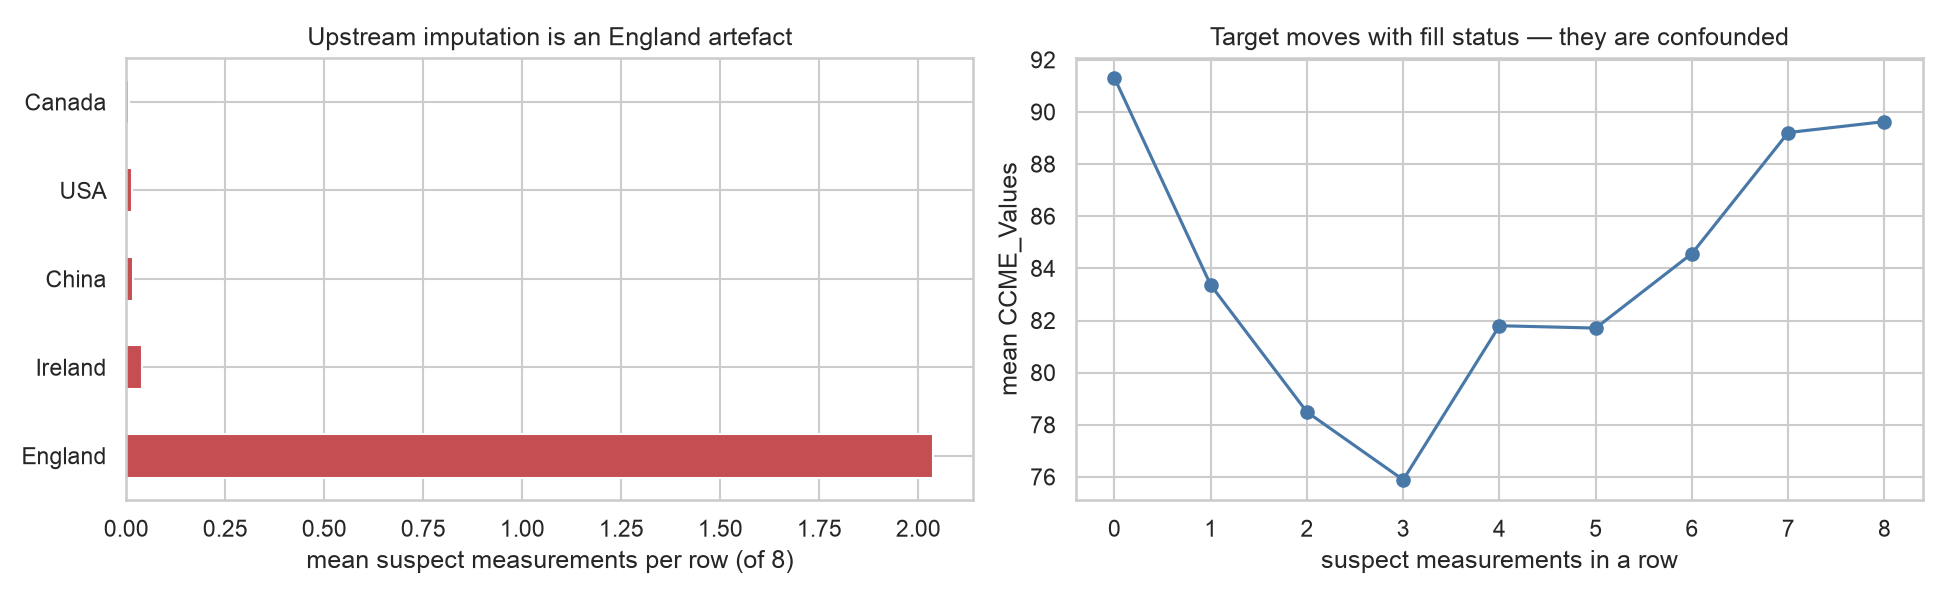
\includegraphics[width=\linewidth]{imputation_confound.png}
    \caption{Upstream median imputation is concentrated in one country (left) and is
    confounded with the target (right). Counts at six or more filled measurements are
    small and the apparent recovery there is noise.}
    \label{fig:imputation}
\end{figure}

\subsection{A Bounded Target with a Mass at the Ceiling}
\label{sec:ceiling}
The index is bounded above at 100 and 35.92\% of records sit exactly at that bound; the
75th, 90th and 99th percentiles are all 100 (Fig.~\ref{fig:target}). The distribution has
no upper tail, only a spike. The share at the ceiling varies from 20.9\% (England) to
84.5\% (USA), so the target's shape differs by country. Residuals above the ceiling are
impossible by construction, making errors asymmetric.

We describe this as a bounded target with a point mass rather than a censored one, and
the distinction matters for how it should be modelled. Censoring implies a latent value
beyond the observation threshold that the recording process conceals. Here there is no
latent value: by Equation~\eqref{eq:ccme}, a record for which every measurement meets its
guideline yields $F_1 = F_2 = F_3 = 0$ and therefore exactly 100. The ceiling is a
property of the index's construction, not of its measurement, so Tobit-style censored
regression is not the appropriate remedy. What the mass does imply is that the task
mixes two questions -- whether a record is fully compliant, and how far from compliance
it falls otherwise -- which a single pooled error statistic reports as one number.

\begin{figure}[!t]
    \centering
    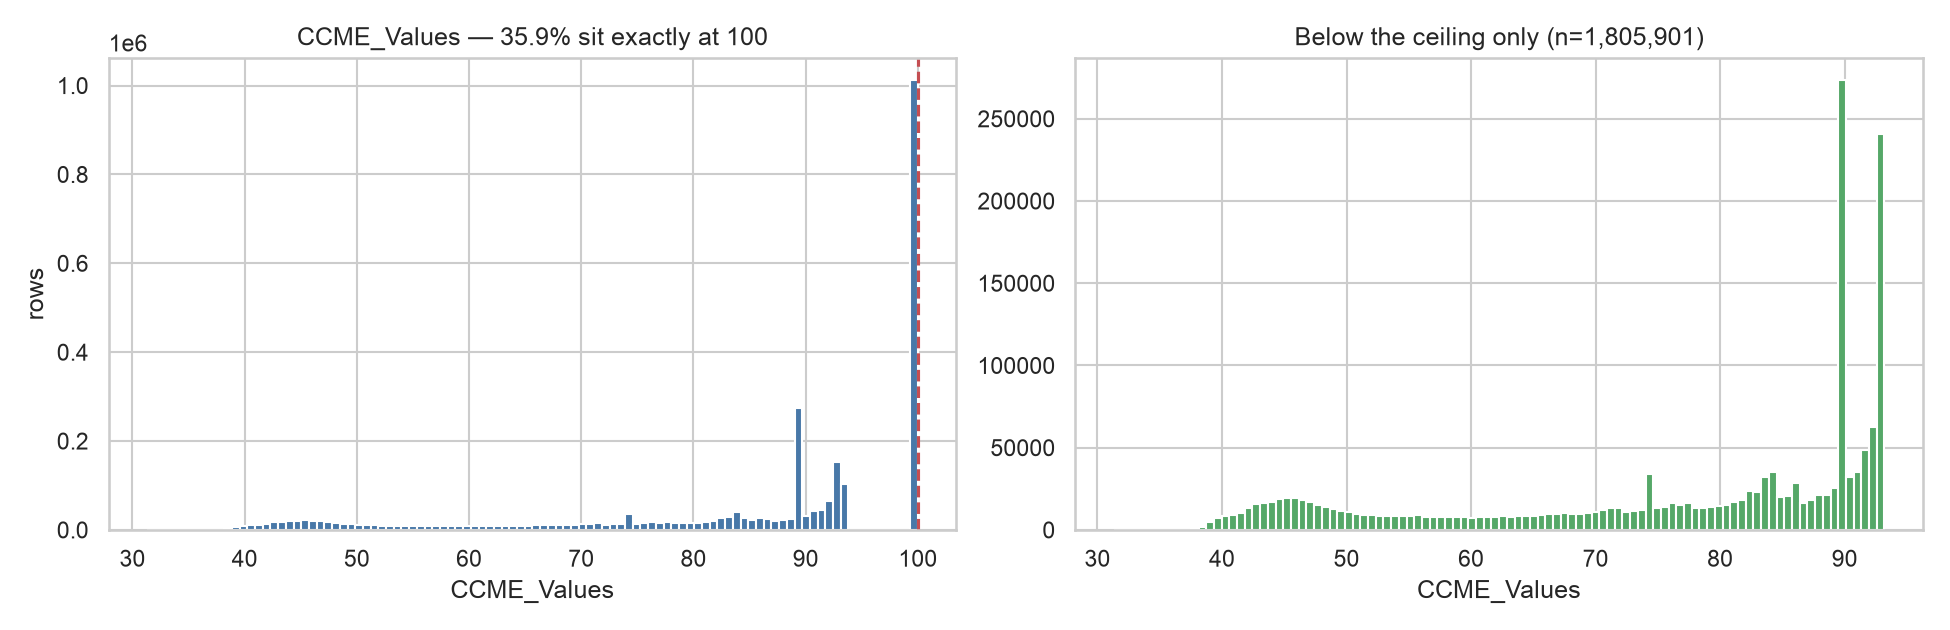
\includegraphics[width=\linewidth]{target_distribution.png}
    \caption{The CCME index is bounded at 100, where 35.92\% of records sit exactly
    (left); the distribution below the ceiling is shown at right.}
    \label{fig:target}
\end{figure}

\subsection{Distributional Properties}
The measurements are strongly right-skewed: ammonia reaches a skewness of 11.98 with
kurtosis 222, BOD 10.21 and orthophosphate 8.94. A $\log(1+x)$ transform reduces ammonia
skewness to 3.35. Tree ensembles are invariant to monotone transforms, so this matters
chiefly for the Phase 2 neural model, but we evaluate the transformed features in
ablation regardless.

Orthophosphate attains a Spearman correlation of $-0.917$ with the target, consistent
with its tight guideline threshold dominating the index excursion term. Dissolved oxygen,
by contrast, correlates almost not at all ($r = -0.031$). As dissolved oxygen is a
``more-is-better'' parameter, this suggests the upstream implementation treats its
guideline as an upper bound; we return to this in Section~\ref{sec:limitations}.

Composition is uneven in two further respects. Effluent and sewage account for 22.1\% of
records -- treatment-works outflow rather than natural surface water -- with a mean index
of 66.6 against 90.0 for rivers. And 82\% of records fall between 2000 and 2019, with
England's series beginning only in 2000.
